\documentclass[handout]{beamer}

\usetheme{Frankfurt}
\setbeamertemplate{footline}[frame number]
\setbeamertemplate{navigation symbols}{}
\setbeamertemplate{caption}[numbered]
\setbeamertemplate{caption label separator}[period]

\usecolortheme{beaver}
\setbeamercolor{item}{fg=darkred}
\setbeamercolor{caption name}{fg=darkred}
\setbeamercolor{block title}{bg=darkred, fg=white}
\setbeamercolor{block body}{bg=gray!10, fg=black}

\urlstyle{same}
\def\arraystretch{1.5}
\def\singleitem#1{\begin{itemize}\item #1\end{itemize}}
\def\red#1{\textcolor{red}{#1}}

% PACKAGES -----------------------------------------------------------------------------------------

\usepackage{graphicx}
\usepackage{ragged2e}
\usepackage{booktabs} 
\usepackage{tikz}

% BIBLIOTECAS TIKZ NECESSÁRIAS PARA O DIAGRAMA -----------------------------------------------------
\usetikzlibrary{positioning, fit, shapes.geometric, arrows.meta, backgrounds}

% DOCUMENT INFORMATION -----------------------------------------------------------------------------

\title
    [LLM Checkpointing]
    {CHORUS: Checkpoint Orchestration with Rate-limiting and Unified Service-policies}
\subtitle{\color{black} \small Advanced Computing Project 25/26}

\author[André Miranda, Gustavo Barros, José Soares, Miguel Carvalho]{
    \scriptsize
    \begin{tabular}{lc}
        André Miranda   & \color{gray} PG60238    \\
        Gustavo Barros  & \color{gray} PG61527    \\
        José Soares     & \color{gray} PG60277    \\
        Miguel Carvalho & \color{gray} PG61153
    \end{tabular}
}

\institute[DIUM]{Department of Informatics -- School of Engineering -- University of Minho}

\date[2026/06/02]{\scriptsize June 02, 2026}


% Document Content ---------------------------------------------------------------------------------

\begin{document}

\frame{\titlepage}

\begin{frame}{Table of contents}
    \tableofcontents
\end{frame}

\section{Introduction}
\begin{frame}{Context \& Problem}
    \small
    \begin{itemize}
        \item \textbf{Context:} LLM training generates massive checkpoints (GBs to TBs).
        \item \textbf{The Bottleneck:} Parallel File Systems (PFS) like Lustre suffer from synchronized I/O bursts ("Noisy Neighbor" problem).
        \item \textbf{Consequence:} GPU compute nodes stall while waiting for slow synchronous writes, wasting expensive resources.
    \end{itemize}
    \begin{block}{Central Insight}
        Checkpointing is \textbf{latency-critical for training continuation}, but not for long-term persistence.
    \end{block}
\end{frame}

\section{System Design}

\subsection{Components}
\begin{frame}{System Components}
    \begin{figure}[htbp]
        \centering
        \resizebox{0.95\columnwidth}{!}{%
            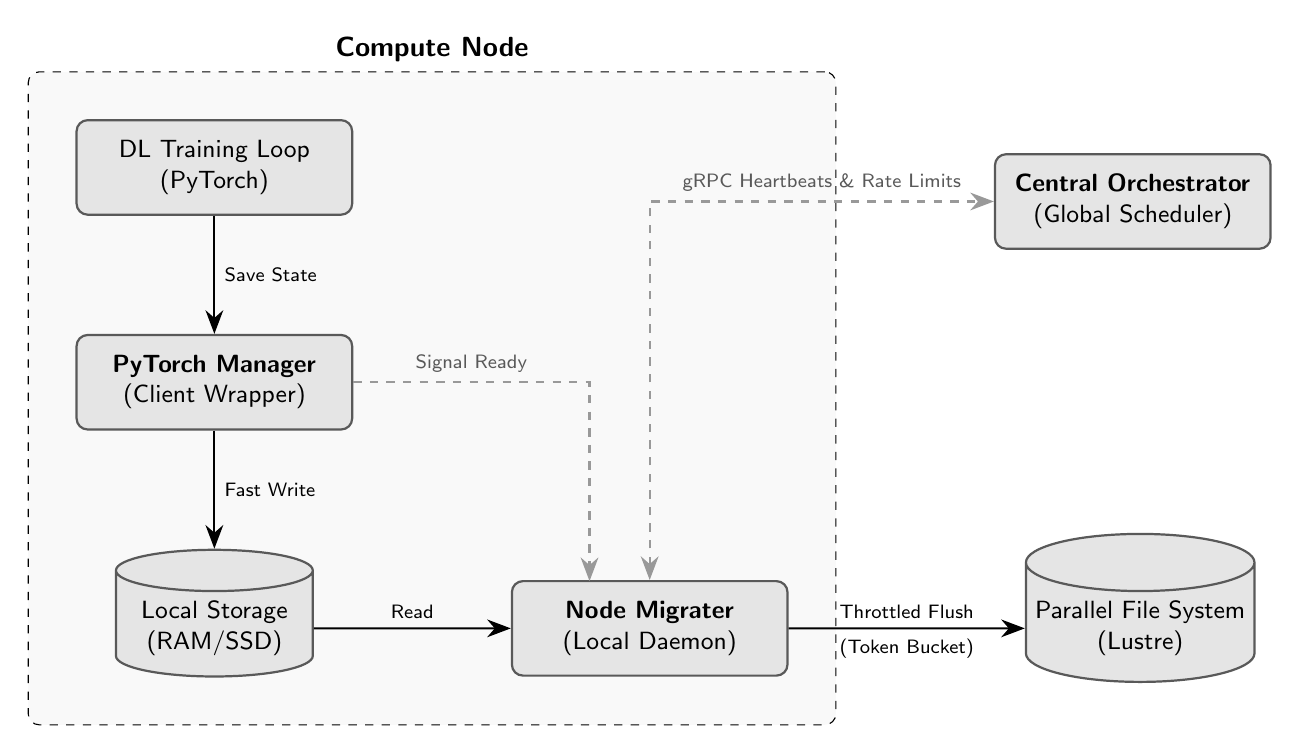
\begin{tikzpicture}[
                node distance = 1.5cm and 2.5cm,
                    box/.style = {draw, rounded corners, minimum width=3.5cm, minimum height=1.2cm, align=center, font=\sffamily\small, thick},
                    database/.style = {cylinder, draw, shape border rotate=90, aspect=0.25, minimum height=1.5cm, minimum width=2.5cm, align=center, font=\sffamily\small, thick},
                    arrow/.style = {-{Stealth[length=3mm]}, thick},
                    grpc/.style = {{Stealth[length=3mm]}-{Stealth[length=3mm]}, dashed, thick, draw=gray!80},
                    signal/.style = {->, dashed, thick, draw=gray!80, -{Stealth[length=3mm]}}
                ]

                \node[box, fill=gray!20, draw=gray!70!black] (train) {DL Training Loop\\(PyTorch)};
                \node[box, fill=gray!20, draw=gray!70!black, below=of train] (manager) {\textbf{PyTorch Manager}\\(Client Wrapper)};
                \node[database, fill=gray!20, draw=gray!70!black, below=of manager] (ssd) {Local Storage\\(RAM/SSD)};
                \node[box, fill=gray!20, draw=gray!70!black, right=of ssd] (migrater) {\textbf{Node Migrater}\\(Local Daemon)};

                \begin{scope}[on background layer]
                    \node[fit=(train)(manager)(ssd)(migrater), draw, dashed, fill=gray!5, inner sep=0.6cm, rounded corners, label={[font=\sffamily\bfseries]above:Compute Node}] (node) {};
                \end{scope}

                \node[box, fill=gray!20, draw=gray!70!black, right=2cm of node, yshift=2.5cm] (orchestrator) {\textbf{Central Orchestrator}\\(Global Scheduler)};
                \node[database, fill=gray!20, draw=gray!70!black, right=3cm of migrater] (pfs) {Parallel File System\\(Lustre)};

                \draw[arrow] (train) -- node[right, font=\sffamily\scriptsize] {Save State} (manager);
                \draw[arrow] (manager) -- node[right, font=\sffamily\scriptsize] {Fast Write} (ssd);
                \draw[signal] (manager.east) -| node[above, near start, font=\sffamily\scriptsize, text=gray!70!black] {Signal Ready} ([xshift=10mm,yshift=6mm]migrater.west);
                \draw[arrow] (ssd) -- node[above, font=\sffamily\scriptsize] {Read} (migrater);
                \draw[arrow] (migrater) -- node[above, font=\sffamily\scriptsize] {Throttled Flush} node[below, font=\sffamily\scriptsize] {(Token Bucket)} (pfs);
                \draw[grpc] (migrater.north) |- node[near end ,above, font=\sffamily\scriptsize, text=gray!70!black] {gRPC Heartbeats \& Rate Limits} (orchestrator.west);

            \end{tikzpicture}
        }
        \caption{System architecture of the framework.}
        \label{fig:architecture}
    \end{figure}
\end{frame}

\subsection{Storage Tiering}
\begin{frame}{Two-Tier Storage Strategy}
    \small
    \begin{columns}
        \begin{column}{0.5\textwidth}
            \textbf{Local SSD Staging:}
            \begin{itemize}
                \item Acts as a "Shock Absorber".
                \item Dedicated, uncontested bandwidth per node.
                \item Decouples training loop from network/PFS latency.
            \end{itemize}
        \end{column}
        \begin{column}{0.5\textwidth}
            \begin{block}{Predictability Result}
                Writing to local SSDs showed \textbf{near-zero variance} in stall times compared to the high volatility of direct PFS writes.
            \end{block}
        \end{column}
    \end{columns}
\end{frame}

\section{Implementation}

\subsection{Policies}
\begin{frame}{Pluggable Scheduling Policies}
    \scriptsize
    \centering
    \begin{tabular}{lp{7cm}}
        \toprule
        \textbf{Policy} & \textbf{Logic} \\
        \midrule
        \textbf{Uniform Fair Share} & Splits bandwidth $B_{\text{PFS}}$ equally among all $N$ nodes, regardless of pending data. \\
        \textbf{Active Fair Share} & Splits bandwidth $B_{\text{PFS}}$ equally among nodes with pending data only. \\
        \textbf{Age Priority}      & Normalized combination of \textit{pending size} and \textit{waiting time} (anti-starvation). \\
        \textbf{Epoch Priority}    & Prioritizes jobs closer to completion (higher training progress $\rho_i$). \\
        \bottomrule
    \end{tabular}
    
    \vspace{1em}
    \small \justifying
    \textbf{Dynamic Control:} Orchestrator sends \texttt{CHANGE\_RATE} or \texttt{HOLD} signals via persistent gRPC streams.
\end{frame}

\subsection{Traffic Shaping}
\begin{frame}{Token Bucket \& Traffic Shaping}
    \small
    \begin{itemize}
        \item \textbf{Mechanism:} Migrater read/write operations consume tokens refilled at the Orchestrator-assigned rate.
        \item \textbf{Chunk Size Tuning:} Evaluated trade-off between throughput accuracy and PFS syscall pressure.
    \end{itemize}
    \begin{exampleblock}{Optimal Configuration}
        \textbf{4 MiB chunks} provided the best balance: high throughput accuracy with significantly reduced write frequency.
    \end{exampleblock}
\end{frame}

\section{Evaluation}

\subsection{Performance}
\begin{frame}{Results: Throughput Profiles}
    % Top Half: 3 Columns with minimal text and no blocks
    \begin{columns}[t]
        \begin{column}{0.33\textwidth}
            \centering
            \footnotesize
            \textbf{Burst Traffic}
            \begin{itemize}
                \item Simultaneous dumps.
            \end{itemize}
        \end{column}
        
        \begin{column}{0.33\textwidth}
            \centering
            \footnotesize
            \textbf{Steady Traffic}
            \begin{itemize}
                \item Staggered intervals.
            \end{itemize}
        \end{column}
        
        \begin{column}{0.33\textwidth}
            \centering
            \footnotesize
            \textbf{Dynamic Churn}
            \begin{itemize}
                \item Job arrivals/departures.
            \end{itemize}
        \end{column}
    \end{columns}

    \begin{center}
        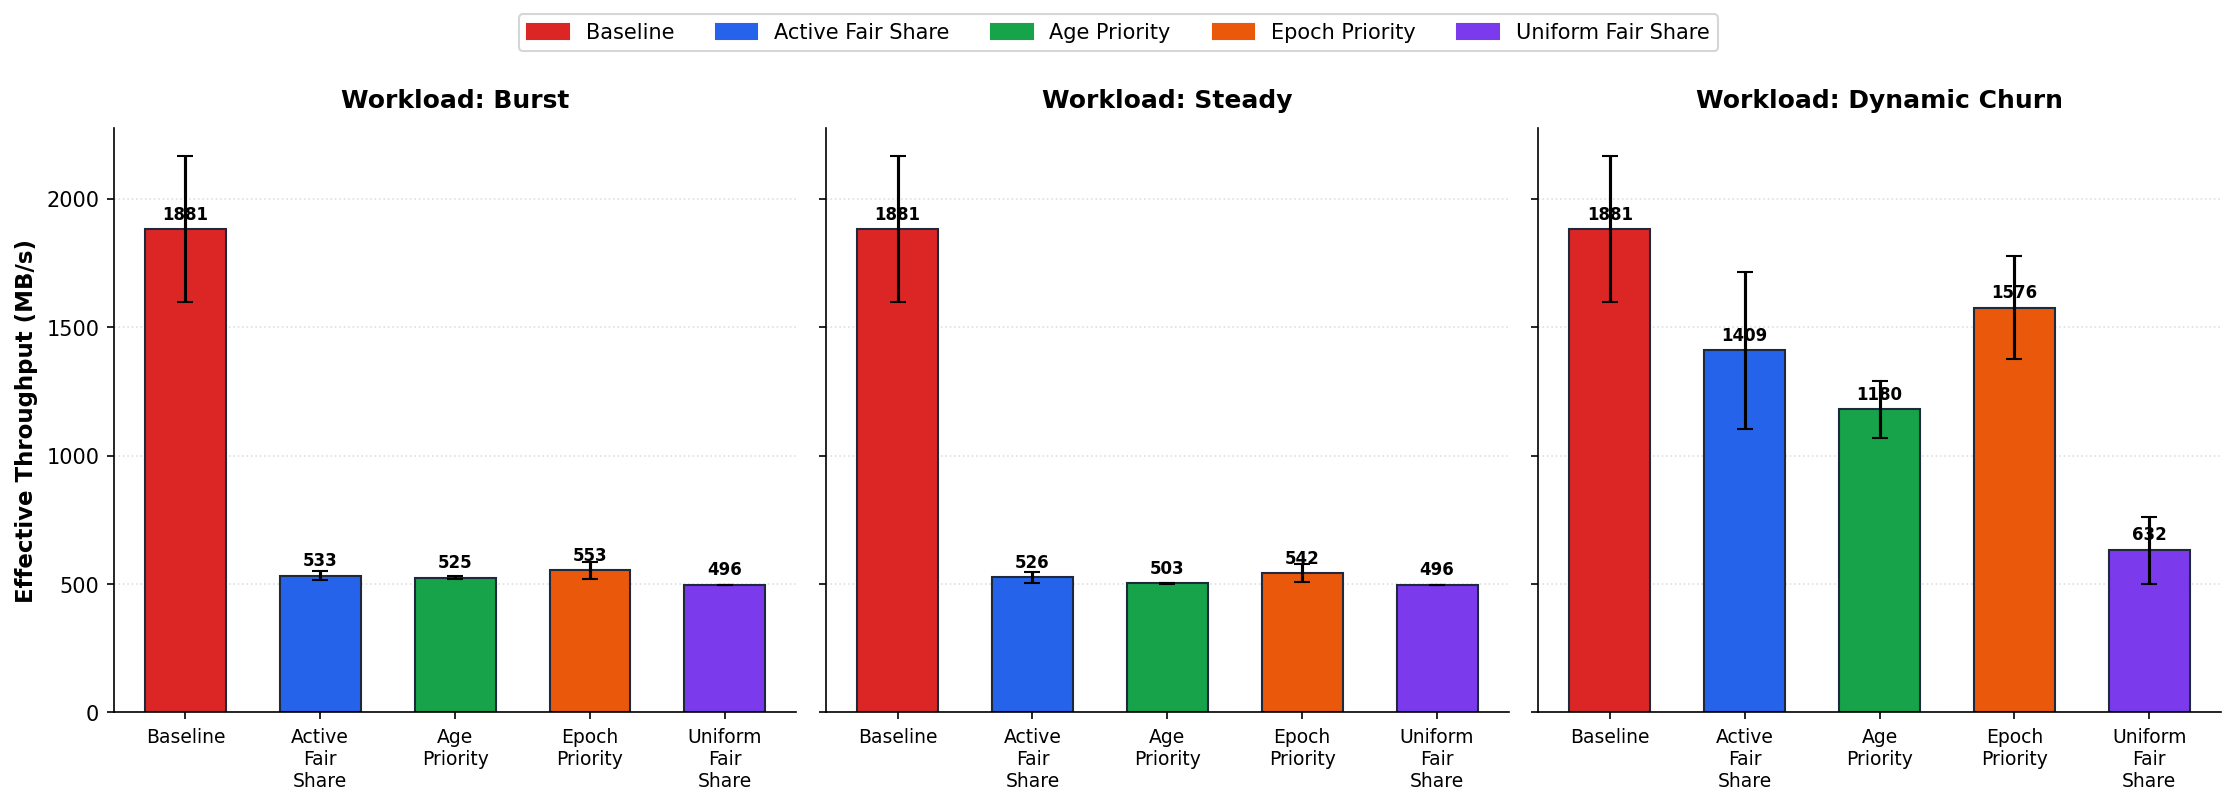
\includegraphics[width=0.9\textwidth]{assets/performance.png}
    \end{center}

    \scriptsize
    \begin{columns}[t]
        \begin{column}{0.5\textwidth}
            \textbf{Setup Parameters:}
            \begin{itemize}
                \item 5 GB checkpoint payload.
                \item 2 GB PFS bandwidth.
            \end{itemize}
        \end{column}
        \begin{column}{0.5\textwidth}
            \textbf{Cluster Environment:}
            \begin{itemize}
                \item Tracked concurrent SLURM jobs to account for shared network background noise.
            \end{itemize}
        \end{column}
    \end{columns}
\end{frame}
\subsection{QoS Enforcement}
\begin{frame}{Bandwidth Convergence}
    \begin{center}
        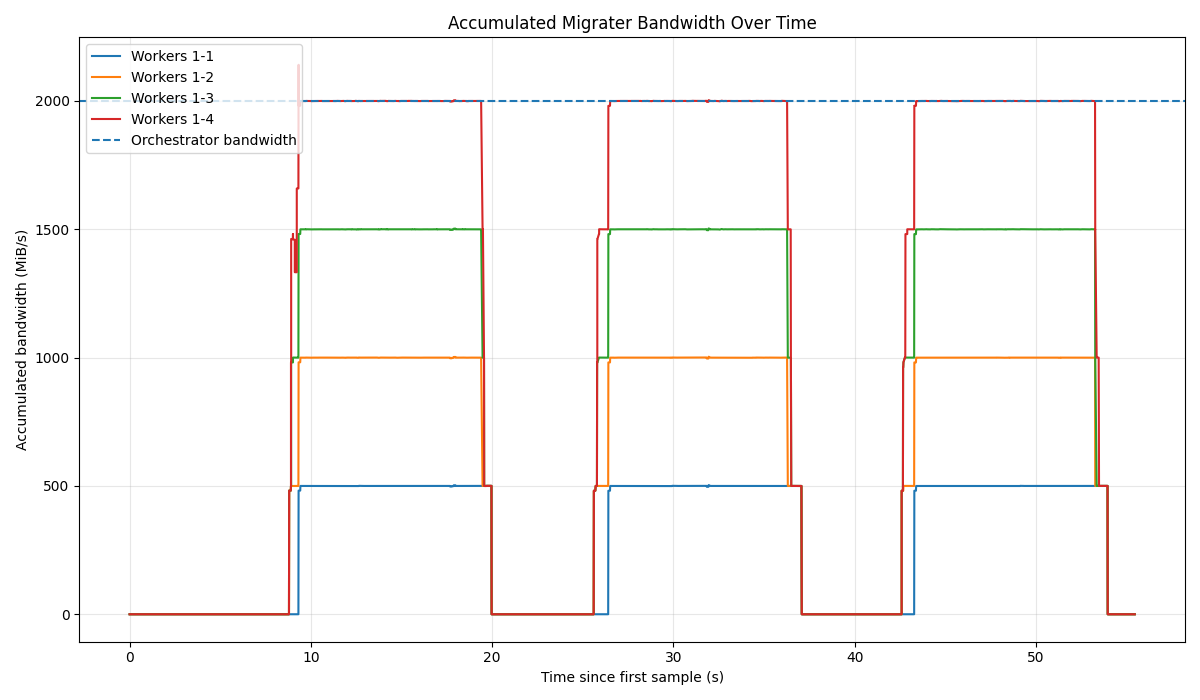
\includegraphics[width=1\textwidth]{assets/bw.png}
    \end{center}
    \begin{center}
        \textit{The system successfully transforms uncoordinated I/O bursts into smooth, regulated storage traffic. However...}
    \end{center}
\end{frame}

\subsection{QoS Enforcement}
\begin{frame}{Bandwidth Convergence (Issues)}
    \begin{center}
        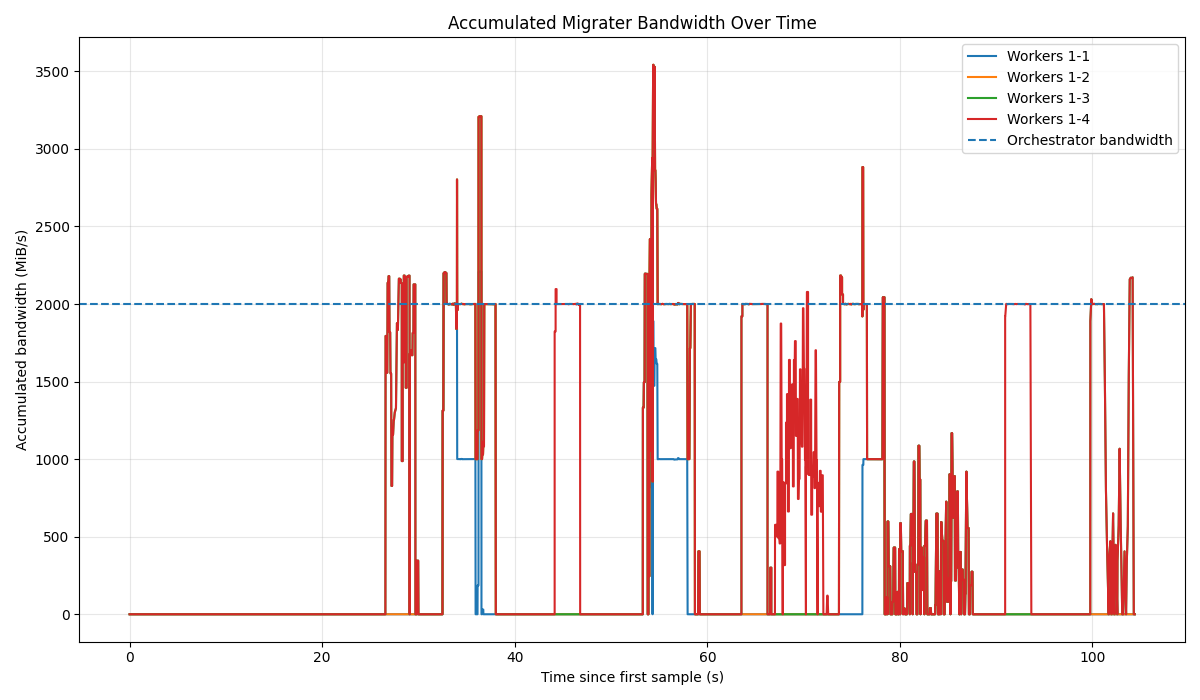
\includegraphics[width=0.85\textwidth]{assets/bad_bw.png}
    \end{center}
    \scriptsize
    \begin{itemize}
        \item \textbf{Signaling Latency Layer:} Caused by the 0.1s gRPC heartbeat sampling stream.
        \item \textbf{Token Accumulation Spikes:} Empty initial bucket balance prevents initial bursts, but sub-second spikes remain at block boundaries.
    \end{itemize}
\end{frame}

\section{Conclusion}

\begin{frame}{Conclusions \& Future Work}
    \small
    \textbf{Conclusions:}
    \begin{itemize}
        \item Two-tier orchestration provides \textbf{predictability} for LLM training.
        \item Centralized rate control ensures \textbf{Cluster Harmony}.
        \item Local SSD staging is a scalable "shock absorber" as hardware evolves.
    \end{itemize}
    
    \vspace{0.5em}
    \textbf{Future Work:}
    \begin{itemize}
        \item \textbf{Exascale:} Stress testing with thousands of concurrent nodes and weak scalability constraints.
        \item \textbf{Non-Blocking Queue Management:} Support queuing or pipelining new checkpoint requests if a worker generates a new state while the previous one is still migrating to the PFS.
        \item \textbf{Resilience:} Fault-tolerant Orchestrator (single point of failure).
    \end{itemize}
\end{frame}

\frame{\titlepage}

\end{document}